\chapter{Alternative SSA construction/destruction algorithms
   \Author{Dibyendu Das, Upadrasta Ramakrishna, Vugranam Sreedhar
                   and F. Rastello}}
\numberofpages{18}
\graphicspath{{img/}{alternative_ssa_construction_algorithms/img/}{part1/alternative_ssa_construction_algorithms/img/}}


%\input defs


%\input defs


\section{Introduction}

The  placement  of $\phi$-functions
is an important step in the construction of Static Single Assignment 
(SSA) form~\cite{CytronEtAl91}.
 In SSA form
 every variable is assigned 
only once. At control flow merge points $\phi$-functions are added 
 to ensure that every use of a variable has exactly 
one definition. 
A $\phi$-function is of the form $x_n = \phi(x_0,x_1, x_2, \ldots, x_{n-1})$,
where $x_i$'s ($i = 0 \ldots n-1$) are a set of variables with static single assignment. 
Consider the example control flow graph where we have shown definitions and uses for 
a variable $x$. The SSA form for the variable $x$ is illustrated in Figure ~\ref{fig:cfg}(a)
without explict renaming. 
Notice $\phi$-functions
have been introduced at certain join (also called merge) nodes in the control flow graph.
In the rest of this chapter we will present three different approaches  for placing $\phi$-functions
at appropriate join nodes. We will begin by introducing concepts of dominance frontiers and
iterated dominance frontiers (IDF). Cytron et al. showed that $\phi$-functions for a set of nodes in the
control flow graph are
placed at exactly the IDF of the set of nodes. Next we present Sreedhar and Gao's algorithm for
placing $\phi$-functions. Sreedhar and Gao's algorithm uses DJ graph representation of a CFG.
Then we will discuss the notion of merge set and merge relation, and present
Das and Ramakrishna's algorithm for $\phi$-functions based on merge relation and using DJ graph. Finally
we describe another approach for placing $\phi$-functions based on loop nesting forest.

\section{Basic Algorithm}
The original algorithm for placing $\phi$-functions
was based on first computing the dominance frontier  (DF) set for the given control flow graph.
The dominance frontier $DF(x)$ of a node $x$ is the set of all nodes 
 $z$ such that $x$ dominates a predecessor of $z$, without strictly dominating $z$.
For example, $DF(8)= \{ 6, 8 \}$ in Figure ~\ref{fig:cfg}(b). A straight forward algorithm for computing
DF for each node takes $O(N^2)$ since the size of the full DF set in the worst case
can be $O(N^2)$.Here $N$ is the number of nodes of the CFG. 
Cytron et al.'s algorithm for the placement of $\phi$-functions consists of computing
iterated dominance frontier (IDF) for a set of all definition points (or nodes where
variables are defined). 
Let $N_{\alpha}$ be the set of nodes where variable $x$ are  defined.
Given that the dominance frontier for a set of nodes is just the
union of the DF of each node, we can compute $IDF(N_\alpha)$ as a limit of
the following recurrence equation (where $S$ is initially $N_\alpha$)
\begin{eqnarray*}
IDF_1(S) &=& DF(S) \\
IDF_{i+1} (S) &=& DF(S \cup IDF_i(S)) 
\end{eqnarray*}

A $\phi$-function is then placed at each join node in the  $IDF(N_{\alpha})$ set. 
Although Cytron et al.'s
algorithm works very well in practice, in the worst case the time complexity of the
algorithm is quadratic in the number of nodes in the original control flow graph.




\section{Placing $\phi$-functions using DJ graphs}
Sreedhar and Gao 
proposed the first linear time algorithm for computing the IDF set without
the need for explicitly computing the full DF set. Sreedhar and Gao's orginal
algorithm was implemented using the DJ graph representation of CFG. A DJ graph
is nothing more than a CFG augmented with dominator tree edges. An edge $x \edge{} y$, of the
CFG, which is not a dominator-tree edge, becomes a join(J) edge The
DJ graph for the example CFG is also shown in Figure ~\ref{fig:cfg}(b). The CFG edge
$10 \edge{} 8$, which is not a dominator-tree edge becomes the J edge, $10 \edge{J} 8$.
Rather than explicitly
computing the full DF set, Sreedhar and Gao's algorithm uses a bottom-up and top-down
traversal of the DJ graph to compute the  $IDF(N_{\alpha})$. Even though
 the time complexity of
Sreedhar and Gao's algorithm is linear, in practice it sometimes performs worse than the Cytron et al.
algorithm. The main reason for this is that in practice the size of the DF set is linear 
and sometimes smaller than the size of the DJ graph. 


\subsection{Key Observation} 
 
Let us try to understand how to compute the DF for a single node using DJ graphs. 
Consider  the DJ graph shown in Figure~\ref{fig:cfg}(b). To compute $DF(3)$ we simply walk down the
dominator (D) tree edges from node 3 and identify all join (J) edges $x \edge{J} y$ such
the $y.level \leq 3.level$, where $level$ of a node is the depth of the node from the
root of the dominator tree. The $level$ of each node is also shown in Figure ~\ref{fig:cfg}(b).
For our example the only J edge that satifies this 
condition is $7 \edge{J} 2$. Therefore the $DF(3) = \{2\}$. To generalize the example, we can
compute the DF of a node $x$ using \\
\fbox{$DF(x) = \{y | z \in SubTree(x) \; \wedge \; z \edge{J} y \; \wedge \; y.level \leq x.level \}$}\\

    \begin{figure}[htb]
    \centerline{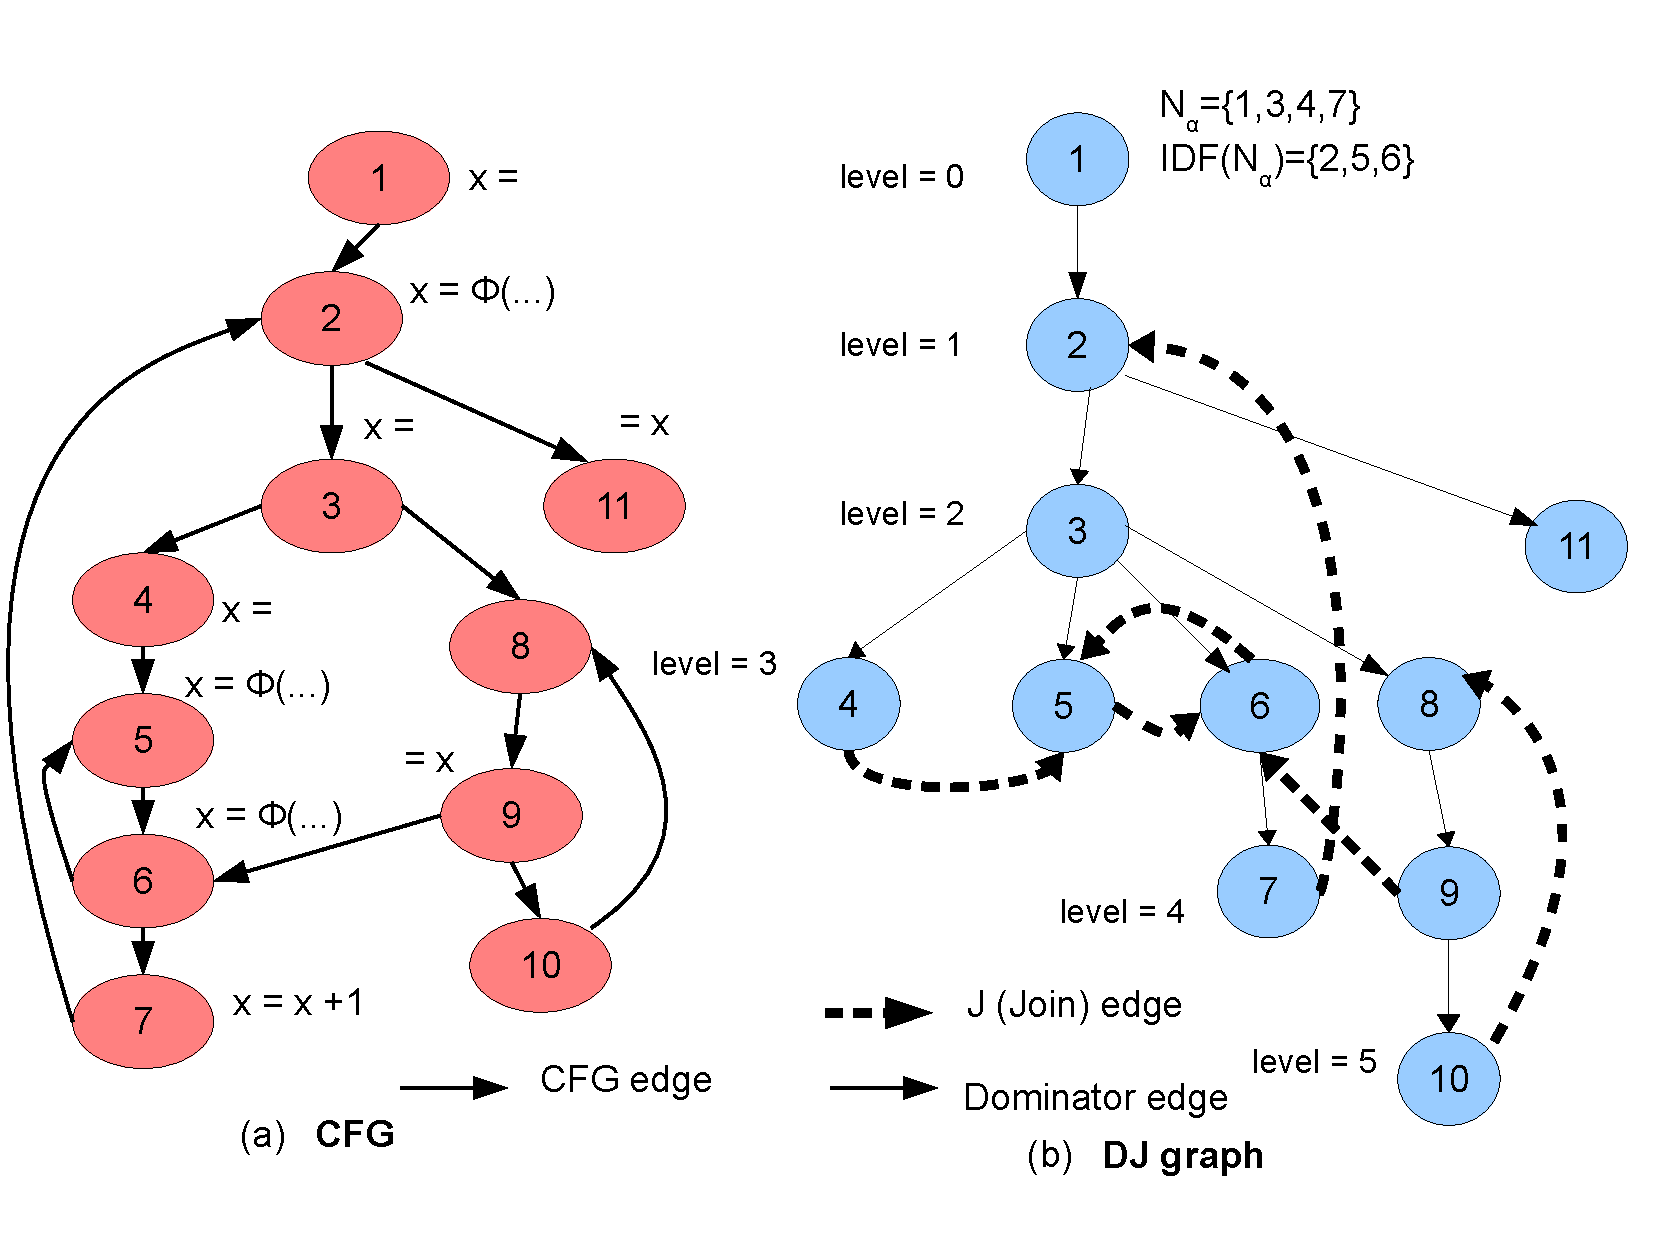
\includegraphics[scale=0.4]{cfglive_new.pdf}}
%    \centerline{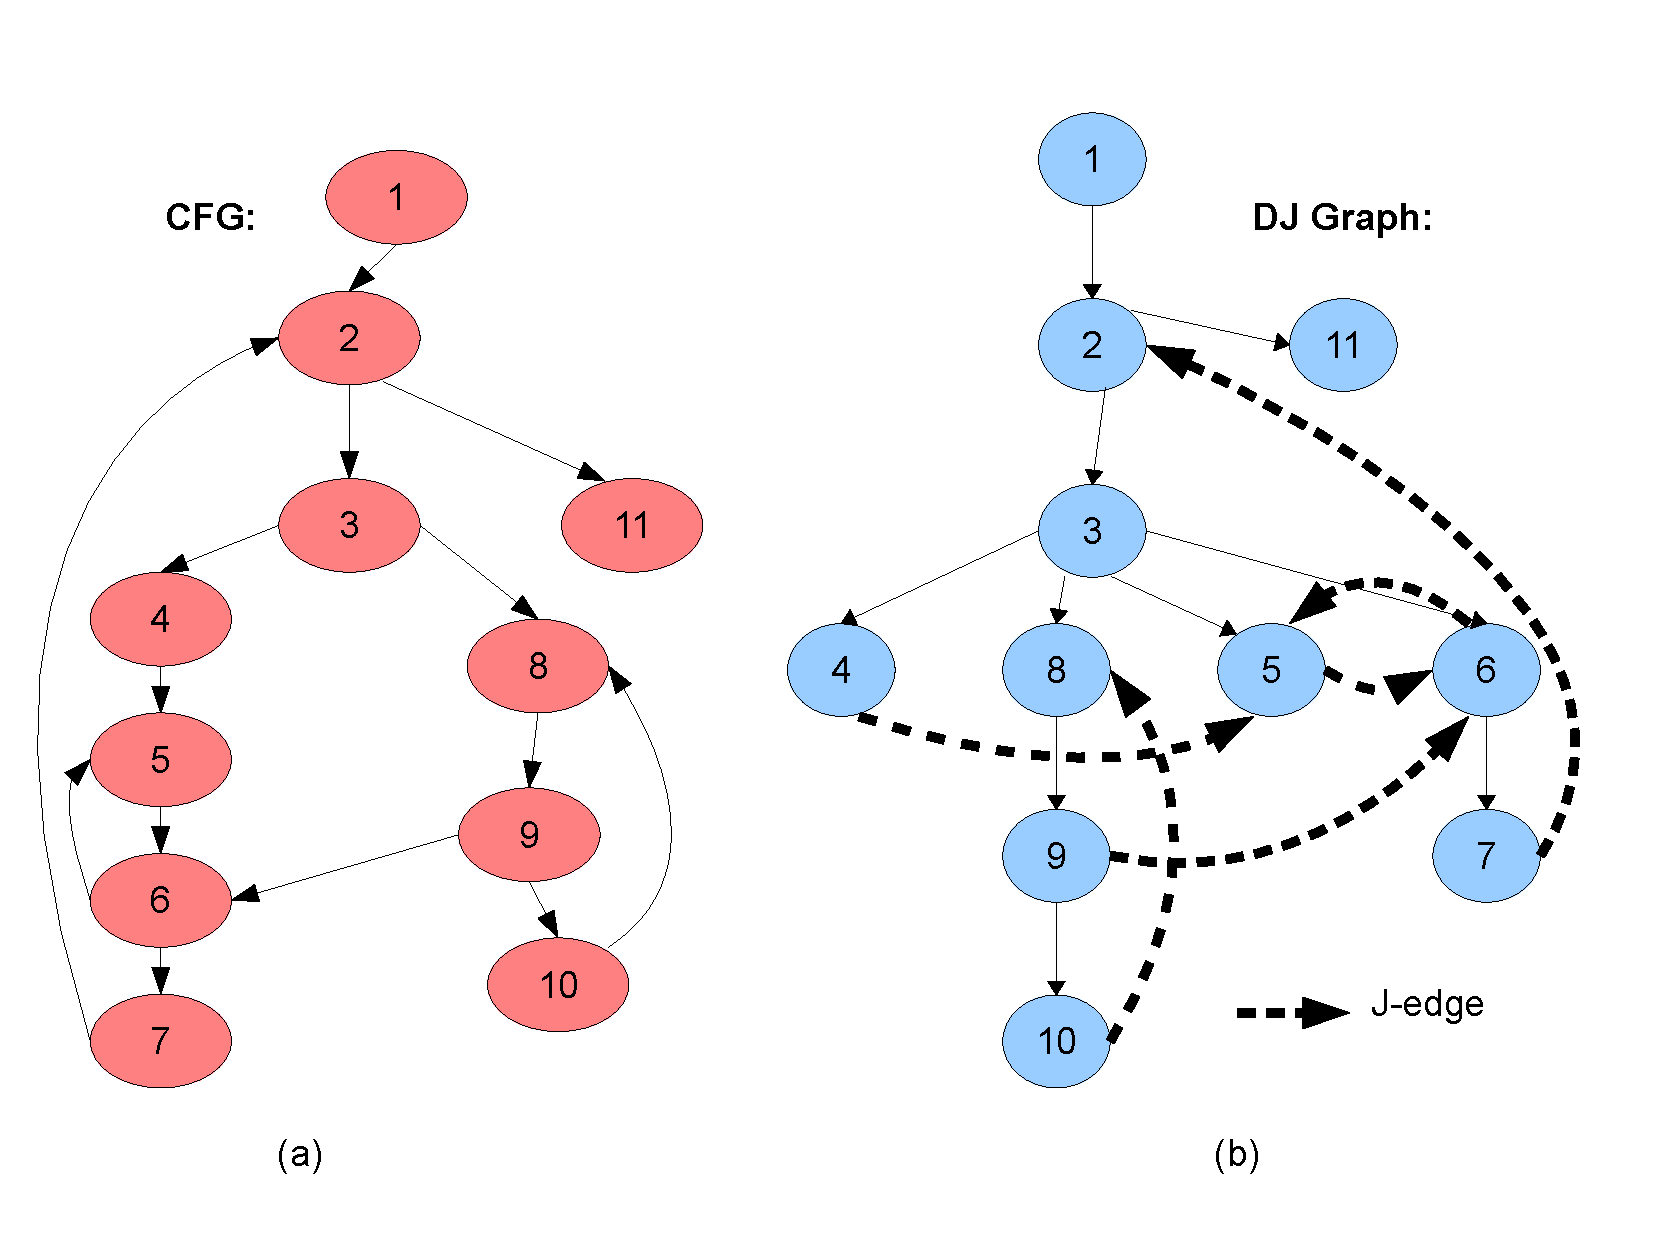
\includegraphics[scale=0.4]{cfglive.pdf}}
    \caption{A Motivating Example (a) CFG (b) DJ graph}
    \label{fig:cfg}
    \end{figure} 

Now we can extend the above idea to compute the IDF for a set of nodes, and hence
the set of $\phi$-functions. Given a set of initial nodes $N_{\alpha}$ to compute the 
relevant set of $\phi$-functions,
Sreedhar and Gao  made two key observations: (1) Let $y$ be an ancestor node of a node $x$ 
on the dominator tree. If $DF(x)$ has
already been computed before the computation of $DF(y)$,  $DF(x)$ need not
be recomputed when computing $DF(y)$. However, the reverse may not be
true, and  therefore the order of the computation of DF is crucial. 
(2) When computing $DF(x)$ we only need to examine J edges $y\edge{J} z$, where $y \in SubTree(x)$
and $z$ is a node such that $z.level \leq x.level$.

To illustrate the two key observations consider the example DJ graph in Figure \ref{fig:cfg}(b),
and let us compute $IDF(\{8,9\})$. Now supposing we start with node 8 and compute 
$DF(8)$ using the second key observation. The resulting DF set is $DF(8) = \{6,8\}$. 
Now supposing we next compute the DF set for node 9, and the resulting set is
$DF(9) = \{6,8\}$. Notice here that we visited the edges $9 \edge{J} 6$ and
$9 \edge{J} 6$ twice, once during the computation of $DF(8)$ and once again
during the computation of $DF(9)$. We can avoid such duplicate visits using the
first key observation by ordering the computation of DF set so that we first compute
$DF(9)$ and then during the computation of $DF(8)$ we avoid visiting the sub-tree of
node 9, and use the result $DF(9)$ that was previously computed. In the next section
we present the Sreedhar and Gao's algorithm based on the above key observations.


\subsection{Main Algorithm}

In this section we present Sreedhar and Gao's algorithm. Let $x.level$ be the
depth of the node from the root node with $root.level= 0$. To ensure that the nodes
are processed according to the first key observation we use  a simple 
 array of sets $OrderedBucket$, and two functions defined over the array of sets:
(1) InsertNode($n$) that inserts the node $n$ in the set $OrderedBucket[n.level]$, and
(2) GetNode() that returns a node from the $OrderedBucket$ with highest level number. 
The complete Sreedhar and Gao's algorithm is shown in Figure~\ref{F:IDFMain}.

\begin{figure}[!ht]
\centering
\begin{minipage}[t]{5in}
\noindent{\bf Input:} A DJ graph representation of a program and $N_{\alpha}$.
\noindent{\bf Output:} The set $IDF(N_{\alpha})$.

Procedure IDFMain(Set $N_{\alpha}$) 
\{
\begin{code}
\x1 $IDF = \{ \}$
\x1 {\bf foreach} ( node $x \in  N_{\alpha}$) {\bf do}
\x2    InsertNode($x$)
\x1 {\bf end for}
\x1 {\bf while} (($z = GetNode()) \neq NULL$)  \label{C:get}
\x2   $croot = z$
 \x2  $z.visited = true$ ;
 \x2  Visit($z$)
\x1 {\bf end while}
\end{code}
\} 

Procedure Visit($x$)
\{
\begin{code}
\x1 {\bf foreach} (node $y \in  Succ(x)$) {\bf do}
\x2  {\bf if} ($x \edge{} y$ is a  J edge) {\bf then}
\x3   {\bf if} ($y.level \leq croot.level$) {\bf then}

\x4     {\bf if} ($y \not \in IDF$) {\bf then}
\x5        $IDF = IDF \cup {y}$   \label{C:idf}
\x5        {\bf if} ($y \not  \in N_{\alpha}$) {\bf then}
\x6          InsertNode($y$) \label{C:insert}
\x5        {\bf endif}
\x4     {\bf end if}
\x3  {\bf end if}
\x2 {\bf else} // visit D edges 
\x3   {\bf if} ($y.visited == false $) {\bf then}
\x4    $y.visited = true$
\x4    // if($y.boundary == false$)   \label{C:cached}
\x5     Visit($y$) \label{C:dedges}
%\x4     Visit($y$) \label{C:dedges}
\x4 // {\bf end if}
\x3   {\bf end if}
\x2  {\bf end if}
\x1 {\bf end for}
\end{code}
\} 
\end{minipage}
\caption{Sreedhar and Gao's algorithm for computing IDF set.}
\label{F:IDFMain}
\end{figure}

First we insert all nodes in $N_{\alpha}$ in the $OrderedBucket$. The nodes are processed
in a bottom-up fashion over the dominator tree from highest node level to least node level
(step ~\ref{C:get}). The procedure Visit($x$) essentially walks down the  DJ graph 
and identifies candidate J edges whose destination node are in the $IDF$ set (step \ref{C:idf}).
Notice that at step \ref{C:insert} a node is inserted in the {\it OrderedBucket} if it was
never inserted before. Finally at step \ref{C:dedges} we continue to process the nodes
in the sub-tree by visiting over the D edges. When the algorithm terminates the 
set $IDF$ will contain the IDF set for the initial $N_{\alpha}$.

    \begin{figure}[htb]
    \centerline{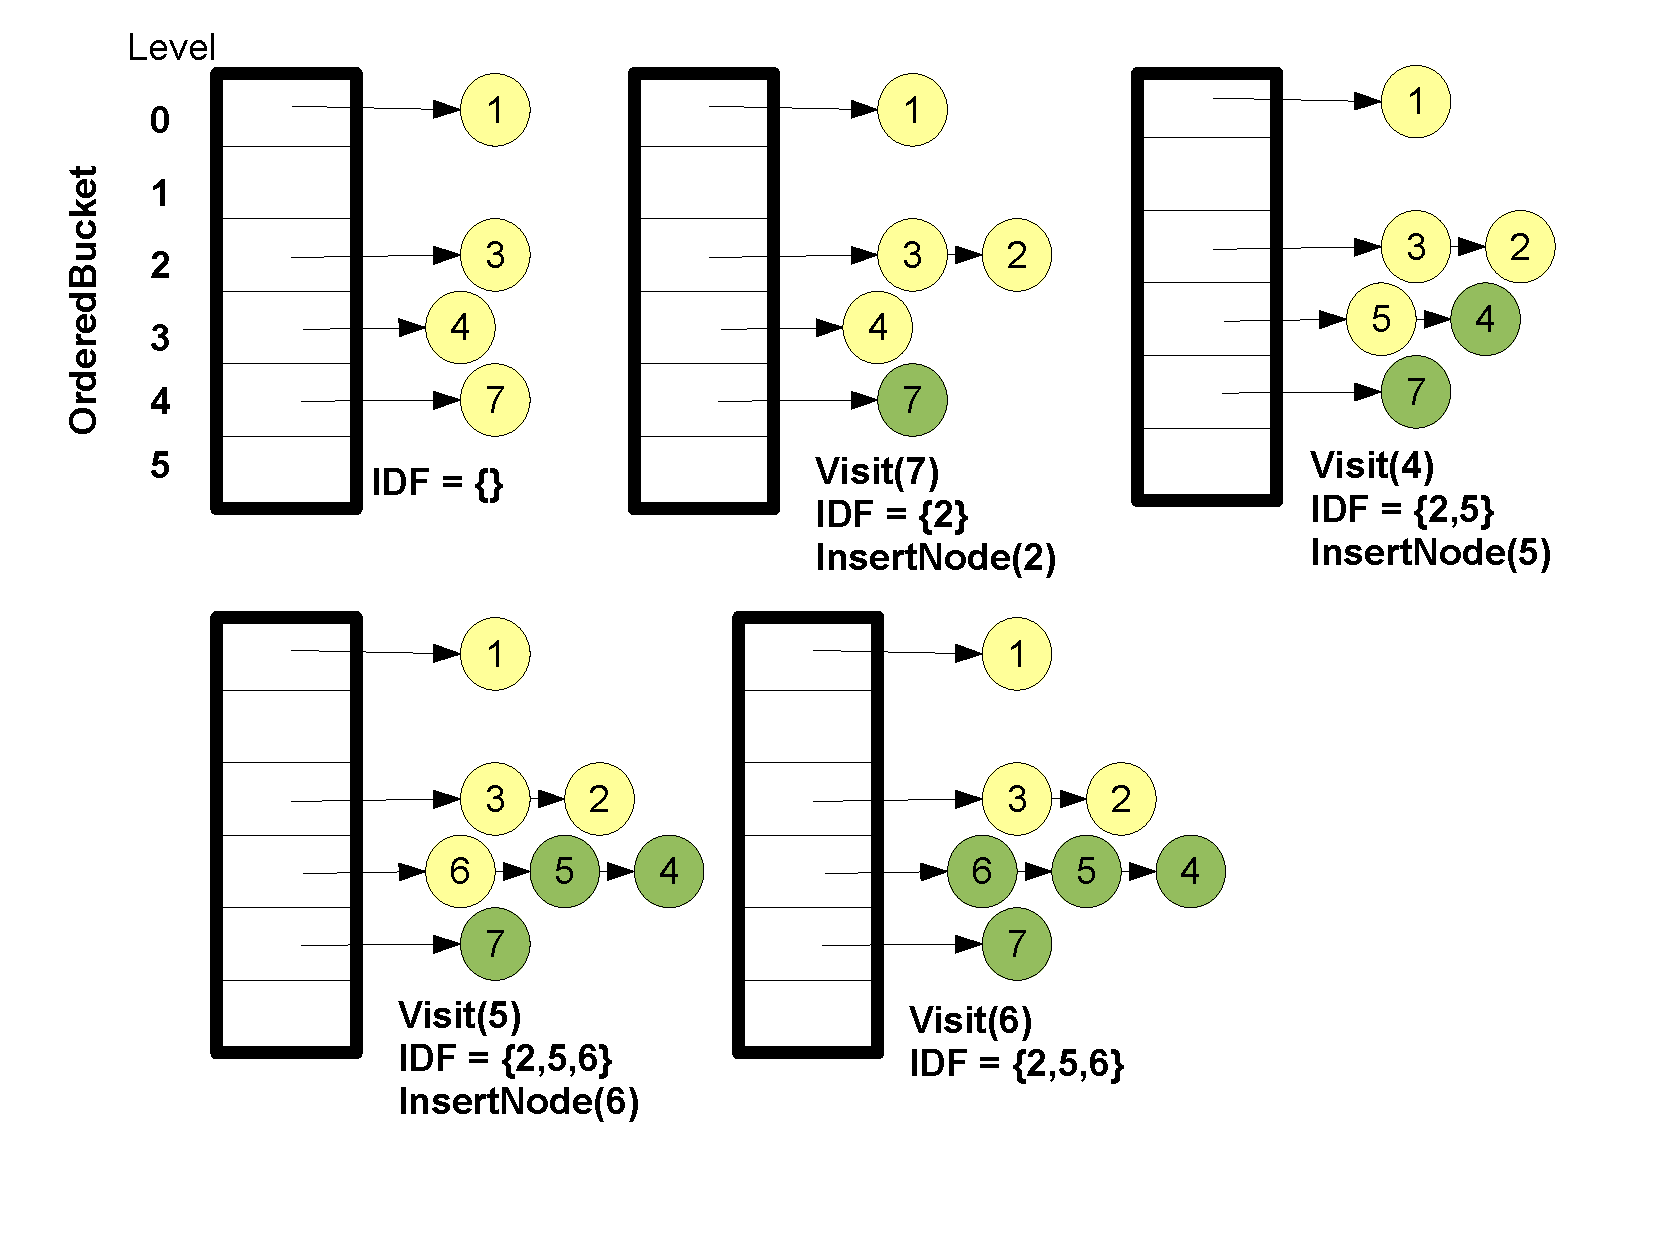
\includegraphics[scale=0.3]{sreedhargao.pdf}}
    \caption{Phases of Sreedhar and Gao's algorithm for $N_\alpha=\{1,3,4,7\}$.}
    \label{fig:sreedhargao}
    \end{figure} 

In Figure ~\ref{fig:sreedhargao}, some of the phases of the algorithm are depicted for clarity. The $OrderedBucket$
is populated with the nodes $1,3,4$ and $7$ corresponding to $N_\alpha=\{1,3,4,7\}$. The nodes are
placed in the buckets corresponding to the levels at which they appear. Hence, node 1 which appears at 
level 0 is in the zero-th bucket, node 3 is in the second bucket and so on. Since the
nodes are processed bottom-up, the first node that is visited is node 7. The successor of node 7 is node
2 and since there exists a J edge $7 \edge{J} 2$, and the $IDF$ set is empty, the $IDF$ set is updated
to hold node 2 according to step ~\ref{C:idf} of the Visit procedure. In addition, InsertNode(2) is invoked and 
node 2 is placed in the second bucket. The next node visited is node 4. The successor of node 4 which is node
5 has an incoming J edge $4 \edge{J} 5$ which results in the new $IDF = \{2,5\}$. The final $IDF$ set converges
to $\{2,5,6\}$ when node 5 is visited. Subsequent visits of other nodes do not add anything to the
$IDF$ set. An interesting case arises when node 3 is visited. Node 3 finally causes nodes 9 and 10 also 
to be visited. However, when node 10 is visited, its successor node which is node 8 and which also 
corresponds to the J edge $10 \edge{J} 8$, does not result in an update of the $IDF$ set as the level of
node 8 is higher than that of node 3.

Pingali and Bilardi made one key observation that the DF set 
can be constructed in space and 
time proportional to the number of nodes in the CFG and which supports DF query 
in time proportional to the output size of result of the query.  Pingali and Bilardi used
a representation called APT(Augmented Postdominator Tree) for representing DF set. 
The APT representation can be
thought as cached DJ graph, where J edges are cached at certain points, called 
``boundary nodes'', in the dominator tree. Given the APT 
(or cached DJ graph) of a control flow graph, it is straight forward to 
modify  Sreedhar and Gao's algorithm for computing $\phi$-functions in linear time. 
 The only modification that is needed is to
ensure that we need not visit all the nodes of a sub-tree rooted at a node
$y$. At step \ref{C:cached} if a node $y$ is a boundary node, we avoid visiting 
the subtree rooted at $y$. The reason for this is that at a boundary all the
required J edges are cached. 
Finally the time complexity of Sreedhar and Gao's algorithm is linear with respect to the number
of DJ graph edges, each edge in the DJ graph is visited at most
once. Details of cached DJ graph can be found in the next section.



\section{Placing $\phi$-functions using Merge Sets}

In the previous section we described $\phi$-function placement algorithm in terms 
of iterated dominance frontier. There is another way to approach the problem
of $\phi$-function placement using the concept of merge relation and merge set. In this section
we will first introduce the notion of merge set and merge relation and then show
how merge relation is related to DF relation. We will then show how to compute
M (merge) graph using DJ graph and then use M graph for placing $\phi$-functions.

\subsection{Merge Set and Merge Relation}

Let us
define first the notion of a {\em join} set $J(S)$
 for a given set of nodes  $S$ in a control flow
graph.\footnote{In English `join' and `merge' are synonyms, 
but unfortunately
in the literature, due to lack of  better terms, these two synonyms are used to mean
distinct but related concepts.} Consider two nodes $u$ and $v$ and distinct 
paths from $u \edge{+} w$ and $v \edge{+} w$, where $w$ is some node in the CFG. If the 
two paths meet only at $w$ then $w$ is in the join set of the nodes $\{r, u, v\}$,
where  $r$ is the root of the CFG. 
For instance, consider nodes 1 and 9 in Figure ~\ref{fig:cfg}(a).
The paths $1 \edge{} 2 \edge{} 3 \edge{} 8$ and $9 \edge{} 10 \edge{} 8$ meet at $8$ 
for the first time and so $\{8\} \in J(\{1,9\})$. Let $S \subseteq V$ and let
$S_r = S \cup \{root \}$. 
we can compute the join set $J(S_r)$ for all possible pairs $u, v \in S_r$ and determine
all such $w$'s where the two distinct paths $u \edge{+} w$ and $v \edge{+} w$ will
meet for the first time. 

Now let us define {\em merge} relation as a relation $v=M(u)$
that holds between two nodes $u$ and $v$ whenever
$v \in J(\{root, u\})$. We insert a $\phi$-function at $v$ for a variable that is assigned
only at $root$ and $u$. One can show that $J(S_r) = \cup_{u \in S_r} M(u)$. It is 
straight forward to show that for any node $u \in V$, $v \in M(u)$ if and only if
there is a path $u \edge{+} v$ that does not contain $idom(v)$. This relationship between
dominance and merge can be conveniently encoded using DJ graph and used for placing 
$\phi$-functions. First we will construct DF (Dominance Frontier) graph using DJ graph.
For each J edge $u \edge{} v$ in the DJ graph insert a new  $w \edge{J} v$ where
$w = idom (u)$ and $w$ does not strictly dominate $v$. Another way to
look at this is to insert a new J edge $w \edge{} v$ if $w = idom(u)$ and
$w.level \geq v.level$.\footnote{Recall that $w.level$ is the depth of $w$ from
$root$ of the dominator tree.} We repeatedly insert new J edges in a bottom-up fashion
over the DJ graph until no more J edges can be inserted. The resulting
DJ graph is a ``fully cached'' DJ graph, from which we can easily compute
the dominance frontiers for a set of nodes. We will call the fully cached
DJ graph as the DF graph. Figure ~\ref{fig:mgraph}(a) shows the DF graph
that is derived from the DJ graph. Notice that for the J edge $10 \edge{J} 8$, additional
J edges are inserted for the DF graph. These are $9 \edge{J} 8$ and $8 \edge{J} 8$ respectively.
Given the DF graph we can compute
the dominance frontier as $DF(u) = \{ v | u \edge{J} v\}$.


Next we can compute the M relation easily from the DF graph. 
Recall that  we insert an edge from a node $u$ to
a node $v $ if $v \in M(u)$. Using DF graph we compute
the M graph as transitive closure
using only the J edges. Now given the M graph of
a CFG we can place $\phi$-functions to a set $S \subseteq \ V$ at the neighbouring nodes
of the nodes in $S$. In other words for each node $u \in S$ we place a $\phi$-function
at $v$ if $u \edge{J} v$ in M graph. Figure ~\ref{fig:mgraph}(d) shows the M graph 
where the merge sets $M(x)$ for each node $x$ is shown.
For node 8, $M(8) = \{2,5,6,8\}$, as the transitive closure on the DF graph results in
the nodes $2, 5, 6$ and $8$ becoming reachable from node 8 via J edges. 

It can also be shown that the merge, join and IDF are equivalent. Thus, for a node $x$,
$M(x) = IDF(x) = J(x \cup \{root\})$.


    \begin{figure}[htb]
    \centerline{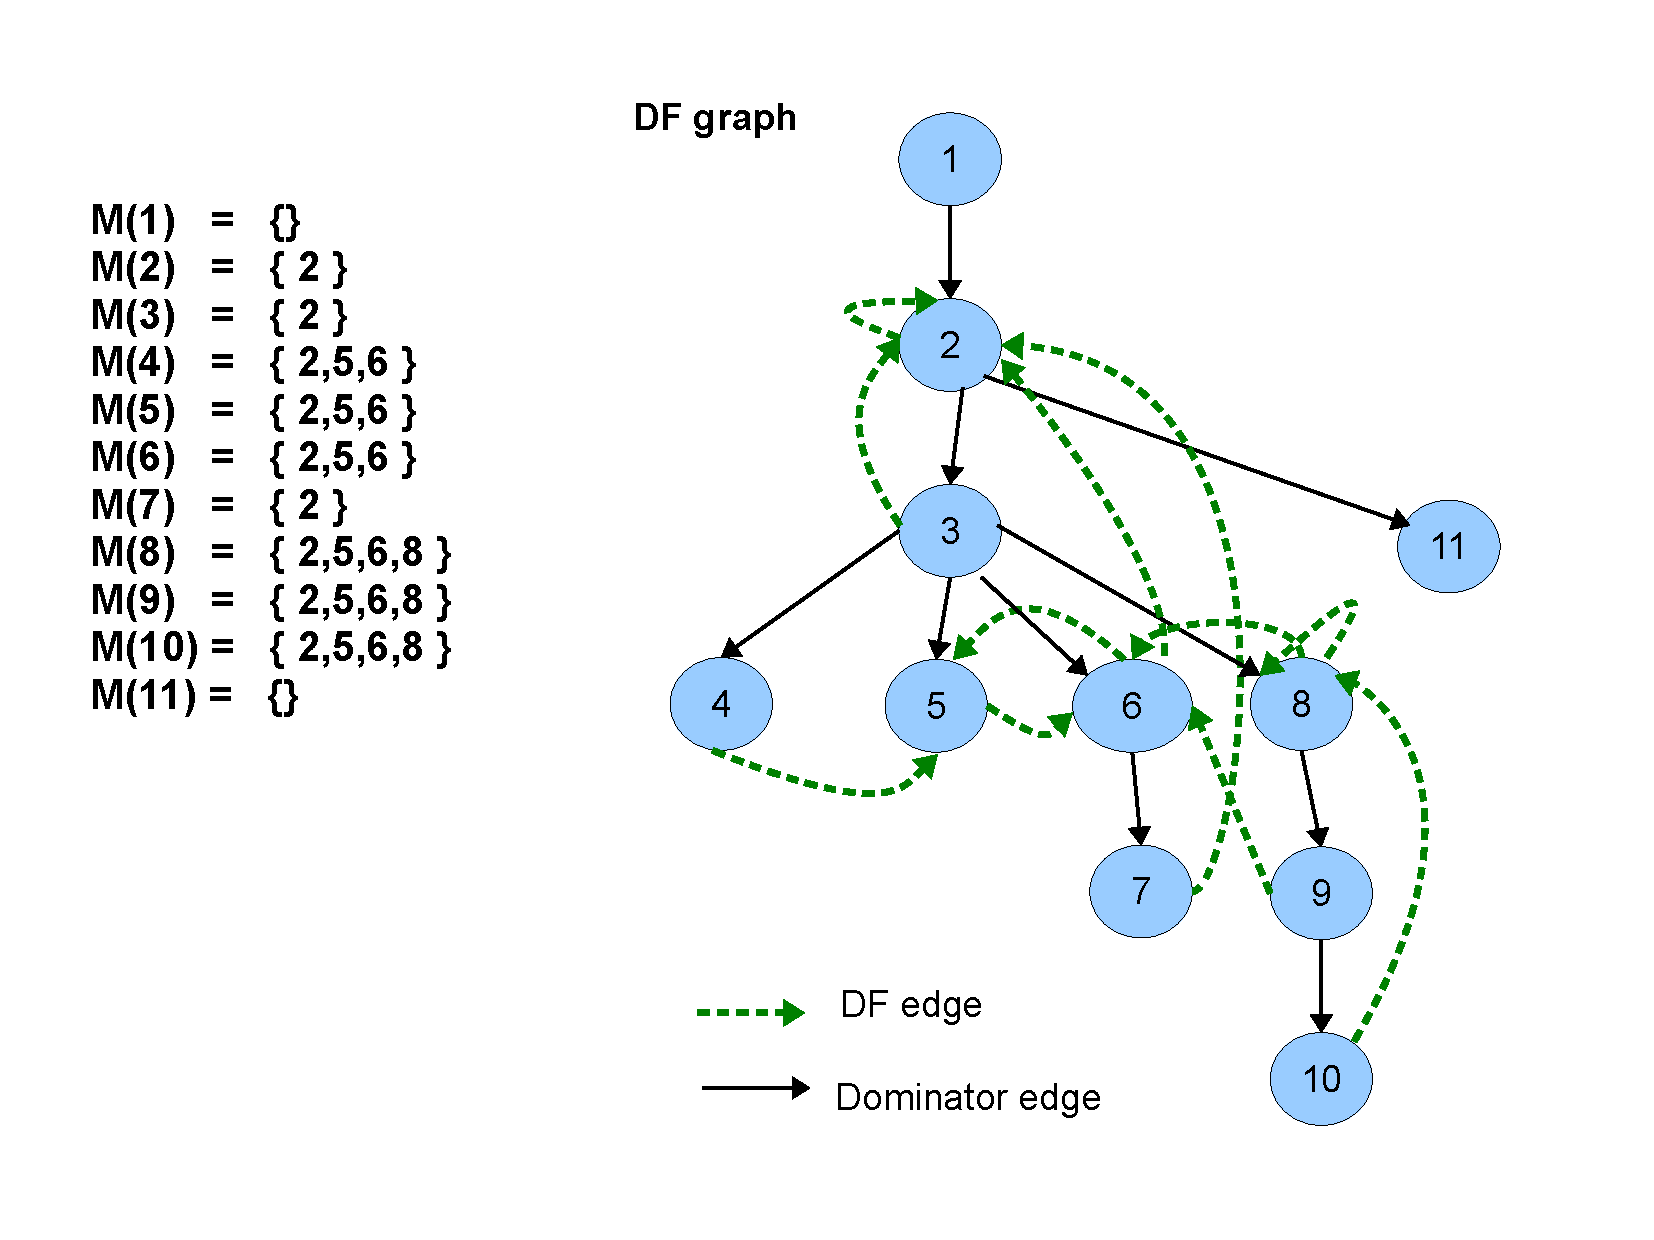
\includegraphics[scale=0.4]{mgraph_1.pdf}}
    \caption{(a)DF-graph/$\omega$-DF graph (b)$\omega$-DJ graph (c) $\gamma$-DJ graph (d)M graph}
    \label{fig:mgraph}
    \end{figure} 


\subsection{Reduced DJ graph}

The algorithm for placing $\phi$-functions based on the construction of DF graph or M graph 
in the worst case can be quadratic. In this section we will describe an approach for
computing $\phi$-functions using reduced DJ graph. Recall that
Sreedhar and Gao's algorithm for computing $\phi$-functions is linear but sometimes perform
worse than the one based on DF graph. Sreedhar and Gao's algorithm is a fully lazy algorithm
in the sense it does not require explicit computation of DF relation. On the
other hand Cytron et al.'s algorithm, which is based on DF graph, explicitly
computes DF graph and then uses this graph to compute the set of $\phi$-functions. 
We can first perform a simple preprocessing step to get rid of
irreducible cycles using DJ graphs as follows: For each J edge $u \edge{} v$
in the DJ graph we insert a new J edge $w \edge{} v$ such that $w.level = v.level$ and
$w$ dominates $u$. We will call the resulting graph as $\omega$-DJ graph. 
Figure ~\ref{fig:mgraph}(a) shows that certain edges are marked $\omega$-DF edges. These are the
edges that correspond to DF when the source and the target nodes are at the same level as
defined in \cite{bilardi}. The
$\omega$-DJ graph shown in Figure ~\ref{fig:mgraph}(b) is an augmented DJ graph with additional 
edges as described above. It should be noted that the edges marked as $\omega$-DJ edges 
correspond exactly to the ones marked as $\omega$-DF edges in Figure ~\ref{fig:mgraph}(a). 


Now given  the $\omega$-DJ graph we collapse all strongly connected cycles of J edges whose
source and destination nodes are at the same level. In other words, find all
strongly connected cycles in the $\omega$-DJ graph at a particular level $l$  and 
collapse them and create a representative  node $s$ at level $l$. 
Let $rep(s)$ denote the set of nodes for which $s$ is the representative node at a 
particular level. Now let $t \in rep(s)$ and consider any outgoing edge
$t \edge{} x$  (either D or J) edges
of $t$. We will insert a new corresponding
(either D or J) edge from $s \edge{} x$. We will process the nodes in the DJ graph
in a bottom-up fashion to construct a reduced DJ graph, which we will call it
as $\gamma$-DJ graph. The $\gamma$-DJ graph in
Figure ~\ref{fig:mgraph}(c) is created by merging the nodes/edges of the $\omega$-DJ graph
when the strongly connected components are folded to single nodes. 
In this case, ignoring the
self-loops for nodes 2 and 8, the nodes 5 and 6 get folded to a single representative 
node (5,6), as nodes
5 and 6 form a strongly connected component in the $\omega$-DJ graph.
Notice that $\gamma$-DJ graph is a reducible graph and so now can efficiently compute
$\phi$-functions using a simpler approach due to Cytron, Lowry, and Zadeck~\cite{xx}.
Ramalingam has given a better exposition of this algorithm which can handle 
reducible graphs. 
 It is important to notice that all nodes in strongly
connected cycles as being equivalent as far as placement of $\phi$-functions is concerned.
Notice that one can also now use Sreedhar and Gao's algorithm on the $\gamma$-DJ graph.


\section{Fast and Practical $\phi$-placement using Merge Sets and DJ graphs}

In this section we describe Das and Ramakrishna's algorithm for placing $\phi$-functions
based on merge relation and using DJ graphs. 
Das and Ramakrishna  made an observation that the $\phi$-functions can be
placed by storing $M(x)$-sets and using
an iterative formulation involving a top-down pass over the DJ-graph.
Empirical observation
suggests that the space complexity of $M(x)$ sets is comparable to that of $DF$-sets
and hence can be used instead of DF to drive the $\phi$- placement.



\subsection{Iterative Merge Set Computation}

The following definition is needed for explaining Das and Ramakrishna's
algorithm.


\paragraph{Shadow:}

Given a J edge $s\edge{J} t$, $Shadow(s\edge{J} t)$ is the set of nodes on the
simple path in the dominator tree from node $idom(t)$ to node $s$,
excluding node $idom(t)$ itself i.e., $\forall x\in Shadow(s\edge{J} t)$,
$x\, dominates\, s$ but does not strictly dominate $t$. 
Consider Figure ~\ref{fig:cfg}(b). Let us consider the J edge $9 \edge{J} 6$.
Here the source node is 9 and the target node is 6. $idom(6)$ is 3. 
$Shadow(9 \edge{J} 6)$ consists of the path $8 \edge{} 9$. Similarly, for $7 \edge{J} 2$
the path is $2 \edge{} 3 \edge{} 6 \edge{} 7$, while for $4 \edge{J} 5$ the 
path consists of only node $5$. Note that the concept of {\it Shadow} is used
(below) to capture the DF values of the nodes and has similarities with the cached-DJ graph mechanism.

The following property of DJ graphs is important for computing the $M(x)$ values of nodes:\\
\fbox{$ \forall x \in V, DF(x) = \bigcup_{s \edge{J} t}\{t|x \in Shadow(s \edge{J} t)\}$}\\
This property points to how the DF value of a node $x$ and the J edges 
are related. The DF value is nothing else but a conglomeration of the target
nodes of the J edges in whose shadow node $x$ lies. Also note that for any target node $t$,
$level(t) \leq level(s)$. Thus, for a node $x$ all the nodes in the $DF(x)$ lie at a level
equal or lower than $x$.
In Figure ~\ref{fig:cfg}(b), $DF(6) = \{2,5\}$ as node $6$ belongs to
$Shadow(7 \edge{J} 2)$ and $Shadow(6 \edge{J} 5)$. Here node $6$ is at the same level as $5$ while
node $2$ is at a lower level.

Since $M(x) = IDF(x) = DF^{+}(x), x \in V$, we can define the merge set for node $x$ by the
following recursive definition : \\
\fbox{$M(x) = DF(x) \bigcup (\cup_{y \in DF(x)} M(y))$ and $level(y) \leq level(x)$} \\
Here, as $level(y) \leq level(x)$, and since we should enumerate the values of $M(y)$,
before we can enumerate $M(x)$, we should visit the nodes top-down in the
DJ graph. Now, we can write, using the above property of $DF(x)$, substituting for $DF(x)$:\\
\fbox{$M(x) = \bigcup_{s \edge{J} t}(\{t|x \in Shadow(s \edge{J} t) \} \cup M(t))$}

We can build up the $M(x)$ values incrementally for each node $x$ lying in the shadow of J edges - as
each J edge is encountered. This is done by capturing the $M(t)$ values of the target nodes of those
J edges and then perforing a union operation with the target nodes for constructing the
corresponding $M(x)$. Thus, if \\
$M^{s \edge{J} t}(x)$ is the contribution of a J edge $s \edge{J} t$ to $M(x)$, then we can write: \\
\fbox{$M^{s \edge{J} t}(x) = \{t\} \cup M(t)$} \\
As, \fbox{$M(x) = \bigcup_{s \edge{J} t}M^{s \edge{J} t}(x)$ }, substituting from above: \\
\fbox{$M(x) = \bigcup_{s \edge{J} t}(\{t\} \cup M(t))$}\\
Thus, $M(9) = \{ 6 \cup M(6) \} \cup \{8 \cup M(8) \}$, since node 9 is in $Shadow(9 \edge{J} 6)$
and in $Shadow(10 \edge{J} 8)$. The $M(6)$ and $M(8)$ values should reach their fixed-points solutions
before $M(9)$ can reach its fixed-point solution. Proceeding top-down over the
dominator tree level by level allows us to compute the $M(x)$ for a node $x$
in a single pass. However, iterative computation may cause multiple passes for cases where
cycles of edges appear in the DF graph at the same level - like the ones involving nodes 5 and 6
in Figure ~\ref{fig:cfg}(b). The cycles are not collapsed( as in the reduced DJ graph case ) as they
may turn out to be costly in some cases.

The following definition is needed to find out whether multiple passes are required for the algorithm.

\paragraph{Inconsistency Condition:}

If the $source(s)$ and $target(t)$ of a $J$-edge do not satisfy
$M(s)\supseteq M(t)$, then the nodes in the shadow of the
$J$-edge are said to be inconsistent. This directly follows from the statement that
$M(s) = \bigcup_{s \edge{J} t}(\{t\} \cup M(t))$, as $s\in Shadow(s \edge{J} t)$.\\

The algorithm described in the next section is directly based on the above method of building
up the $M(x)$ sets of the nodes as each J edge is encountered in an iterative fashion by
traversing the DJ graph top-down. If no node is found to be {\bf inconsistent} after a single 
top-down pass, all the nodes are supposed to have reached fixed-point solutions. If some node
is found to be inconsistent, multiple passes are required till fixed-point solutions can be
reached.

\subsection{TDMSC-I}

%==
\begin{figure}[!ht]
\centering
\begin{minipage}[t]{5in}
\noindent{\bf Input:} A DJ graph representation of a program.
\noindent{\bf Output:} The merge sets for the nodes.

\setcounter{linectr}{0}

Procedure TopDownMergeSetComputation\_TDMSC-I(DJ graph)
\{
\begin{code}
%\textbf{Algorithm: Top Down Merge Set Computation (TDMSC-I)}
%Input: $DJ$-graph
%Outputs: a. Partial/Complete Merge Sets for every node of the DJ graph
%b. A boolean value to indicate whether a subsequent pass is required

\x1 $RequireAnotherPass=False$;

\x1 {\bf while} (in B(readth) F(irst) S(earch) order) {\bf do} \label{C:bfs}
\x2      $n$ $=$ Next Node in BFS list
\x2      {\bf for} (all incoming edges to $n$) {\bf do} \label{C:jedge}

\x3          Let $e = s \edge{J} n$ , be an incoming J edge
\x3          {\bf if} ($e$ not visited) {\bf then}
\x4              Visit($e$) 
\x4              $tmp$ $=$ $s$;
\x4              $lnode$ $=$ $NULL$;
\x4              {\bf while} $(level(tmp)\ge level(t))$ {\bf do} \label{C:mwhiles}

\x5                   $M(tmp)=M(tmp)\cup M(tnode)\cup \{t\}$;
\x5                   $lnode=tmp$;
\x5                   $tmp=parent(tmp)$; //dominator tree parent
\x4              {\bf end while} \label{C:mwhilee}
\x4              {\bf for} (all incoming edges to $lnode$) {\bf do} \label{C:lnode}
\x5                  Let $e'$ $=$ $s^{'} \edge{J} lnode$, be an incoming J edge
\x5                  {\bf if} ($e'$ visited) {\bf then}
\x6                     {\bf if} $(M(s') \not\supseteq M(lnode))$ {\bf then} //Check inconsistency
\x7                         $RequireAnotherPass = True$;
\x6                     {\bf end if}
\x5                  {\bf end if}
\x4              {\bf end for}
\x3          {\bf end if}
\x2     {\bf end for}
\x1 {\bf end while}
\x1 {\bf return} $RequireAnotherPass$;
\end{code}
\}
\end{minipage}
\caption{Top Down Merge Set Computation algorithm for computing Merge sets.}
\label{F:tdmsc}
\end{figure} 

TDMSC-I works by scanning the DJ graph in a top-down fashion as shown in step ~\ref{C:bfs}
using a breadth-first traversal mechanism. This implies that the DJ graph is visited
level-by-level. During this process, for each node $n$ encountered, if there are {\bf incoming}
J edges to $n$ as in step ~\ref{C:jedge}, then a separate bottom-up pass starts at 
step ~\ref{C:mwhiles}. This bottom-up pass traverses the nodes in the $Shadow(s \edge{J} n)$
updating the $M(x)$ values of these nodes. This follows from the contribution of each
J edge $M^{s \edge{J} t}(x)$ to $M(x)$ as discussed earlier. step ~\ref{C:lnode} is used for
inconsistency check. $RequireAnotherPass$ is set to true only if a fixed point is not reached
and the inconsistency check succeeds for some node.

There are some subtleties in the algorithm that should be noted. step ~\ref{C:lnode} of the algorithm
visits incoming edges to $lnode$ only as the the incoming edges to $lnode$'s posterity are at
a level greater than that of node $n$ and are unvisited yet. 

Here, we will briefly walk through TDMSC-I using the DJ graph of Figure ~\ref{fig:cfg}(b).
Moving top-down over the graph, the first J edge encountered is $7 \edge{J} 2$.
As a result, a bottom-up climbing of the nodes happen, starting at node $7$ and
ending at node $2$ and the merge sets of these nodes are updated so that
$M(7) = M(6) = M(3) = M(2) = \{2\}$. The next J edge
to be visited can be any of $4 \edge{J} 5$, $5 \edge{J} 6$ or $6 \edge{J} 5$. Assume it is $5 \edge{J} 6$. This
results in $M(5) = M(6) \cup \{6\} = \{2,6\}$. Now, let $6 \edge{J} 5$ be
visited. Hence, $M(6) = M(5) \cup \{5\} = \{2,5,6\}$. At this point, 
the {\bf inconsistency check} comes into picture for the edge $6 \edge{J} 5$ as $5 \edge{J} 6$
is another J edge that is already visited and is an incoming edge of node $6$.
Checking for $M(5) \supseteq M(6)$ fails, implying that the $M(5)$ needs to 
be computed again. This is done in a separate pass as suggested by the {\it RequireAnotherPass}
value of true. In a second iterative pass, the J edges are visited in the same
order. Now, when $5 \edge{J} 6$ is visited, $M(5) = M(6) \cup \{6\} = \{2,5,6\}$. The
$M(5)$ value is different in this pass as $M(6)$ has become $\{2,5\}$ instead
of just $\{2\}$ in the first pass. On a subsequent visit of $6 \edge{J} 5$, $M(6)$ is
also set to $\{2,5,6\}$. The inconsistency does not appear any more and the algorithm 
proceeds to handle the edges $4 \edge{J} 5$, $9 \edge{J} 6$ and $10 \edge{J} 8$ which have
also been visited in the earlier pass. {\bf TDMSC-I} is invoked repeatedly by a different function
which calls it in a loop till {\it RequireAnotherPass} is returned as $false$.

The algorithm of TDMSC-I is enclosed in another algorithm that repeatedly
calls it till {\bf RequireAnotherPass} is false.


\subsubsection{TDMSC-II}

Das and Ramakrishna term as TDMSC-II, an improvement to algorithm
TDMSC-I. This improvement is fueled by the observation that for an
inconsistent J edge, the merge sets of all nodes in the shadow
of that edge can be locally corrected for some special cases. This
heuristic works very well for certain class of problems -- especially
for CFGs with DF graphs having cycles consisting of a few edges. This
eliminates an extra pass as an inconsistent node is made consistent
immediately on being detected. 

Das and Ramakrishna's TDMSC-II has this additional step immediately
after the inner while loop of TDMSC-I.


%\subsection{Complexity}
%
%A single pass of TDMSC-I can be shown to have a complexity of $O(|V|+|E|)+O(h^{avg}*|J|)+O(e^{avg}*|J|)$.
%For total running time, this has to be multiplied by an additional
%factor of $P$, where $P$ is the number of passes that are needed
%to reach fixed points for merge sets. On average, this overall complexity
%drops down to linear time, if the following factors are taken into
%account: CFGs usually are sparse, both $h^{avg}*|J|$ and $e^{avg}*|J|$
%are of the order of $O(|V|)$, and $P$ is a small constant.



\section{Computing Iterated Dominance Frontier Using Loop Nesting Forests}
    This section illustrates the use of {\bf loop nesting forests} for construction of the iterated
    dominance frontier (IDF) of a set of vertices in a CFG, which may contain both reducible as well as
    irreducible loops.

    \subsection{Loop nesting forest}
     Loop nesting forest is a data structure that respresents the loops in a CFG
    and the containment relation between them. However, while there is a fairly accepted notion of
    loop nesting forest in a reducible graph \cite{morgan_book}, there is less agreement about their
    definition in arbitrary graphs. Steensgard \cite{steensgard}, Sreedhar \cite{sreedhar} and Havlak
    \cite{havlak} all provide different definitions which have merits under different situations. 
    For the example shown in Figure ~\ref{fig:lnf}(a) the loops with backedges $11 \rightarrow 9$ and
    $12 \rightarrow 2$ are both reducible loops. The corresponding loop nesting forest shown in Figure ~\ref{fig:lnf}(b), consists of two loops
    with their header nodes being $2$ and $9$. 
    The loop with header node $2$ contains the loop with header node $9$.

    \begin{figure}[htb]
    \centerline{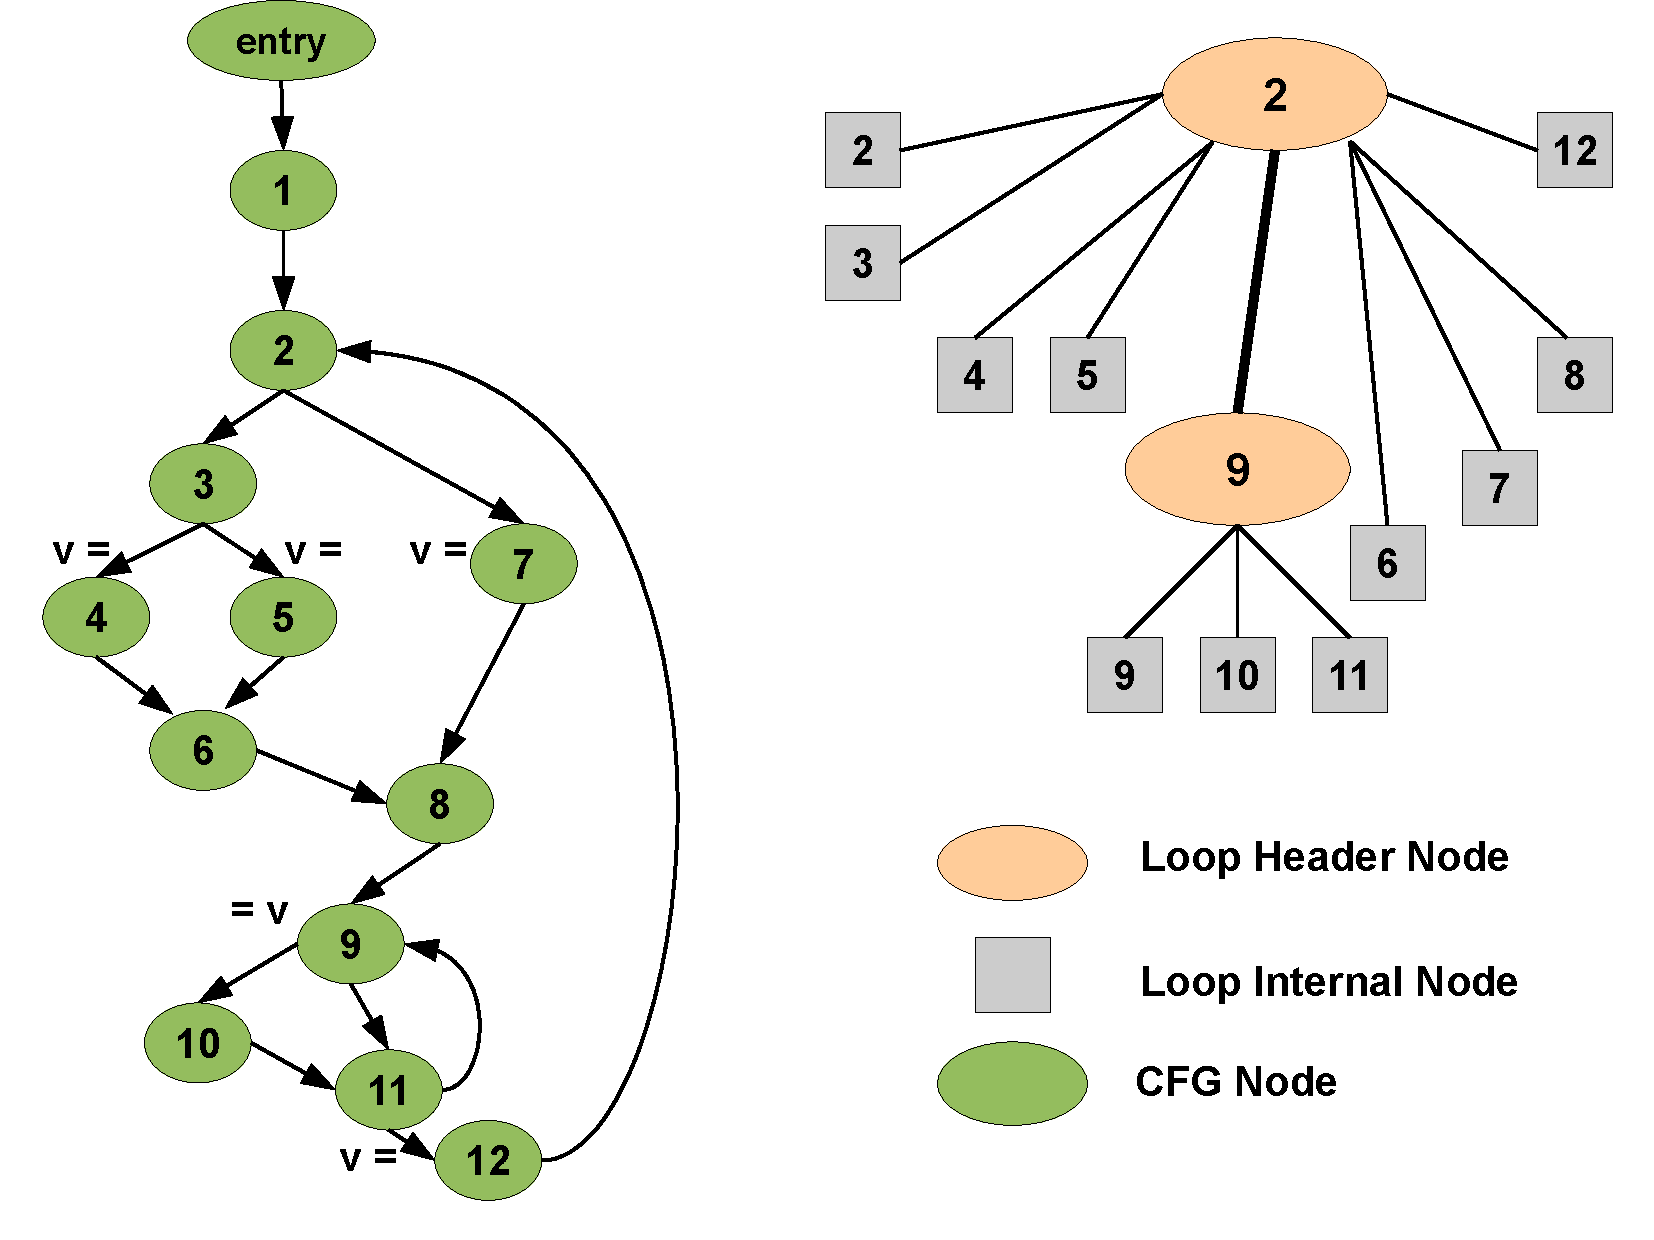
\includegraphics[scale=0.25]{lnfred.pdf}}
    \caption{An example (a) CFG and (b) IDF Computation Using Loop Nesting Forest }
    \label{fig:lnf}
    \end{figure} 


    \subsection{Main Algorithm}
    The IDF for a set of vertices $X$ in an acyclic graph $G_{ac}$, where a certain
    variable $v$ is ``defined'', can be computed as the set of nodes where multiple ``definitions'' of $v$
    reach. Let us say that a definition node $d$ ``reaches'' another node $u$ if there is a path in
    the graph from $d$ to $u$ which does not contain any definition node ( for $v$ ) other than $d$ or $u$.
    Hence, at least one definition node must reach any vertex $u \neq entry(G)$ 
    \footnote{Here $entry(G)$ is a dummy node for all those nodes without predecessors}. If at least two
    definitions reach a node $u$, then $u$ belongs to $IDF(X \cup entry(G))$. 
    This suggests the algorithm in Figure ~\ref{F:ramaIDF} which visits nodes of $G_{ac}$ in
    toplogical order and computes their reaching definitions ( for a variable $v$ ) in step ~\ref{C:rdf}
    or step ~\ref{C:urdf}. If the number of reaching definitions is unique as in step ~\ref{C:onerd},
    then the reaching definition set of the node is updated with the single reaching definition.
    Vertices with more
    than one reaching definition are added to $IDF(X \cup entry(G))$. It should be noted that a 
    vertex is either a definition node or has a unique reaching definition 
    if it is not in $IDF(X \cup entry(G))$.  

    For Figure ~\ref{fig:lnf}, the $G_{ac}$ is formed by dropping
    the backedges $11 \rightarrow 9$ and $12 \rightarrow 2$. Also, $entry(G) = entry$.
    For the definitions of $v$ in nodes $4,5,7$ and $12$ in Figure ~\ref{fig:lnf}, 
    the subsequent nodes where multiple definitions reach turn out to be at $6$ and $8$. For node $6$
    any one of two definitions in nodes $4$ or $5$ can reach. For node $8$, it can be either the
    definition from node $7$ or one of $4$ or $6$.
    Note that the backedges do not exist in the acyclic
    graph and hence node 2 is not part of the IDF set. We will see later how the IDF set for the entire
    graph is computed by factoring in the contribution of the backedges. 



    %\begin{figure}[htb]
    %\centerline{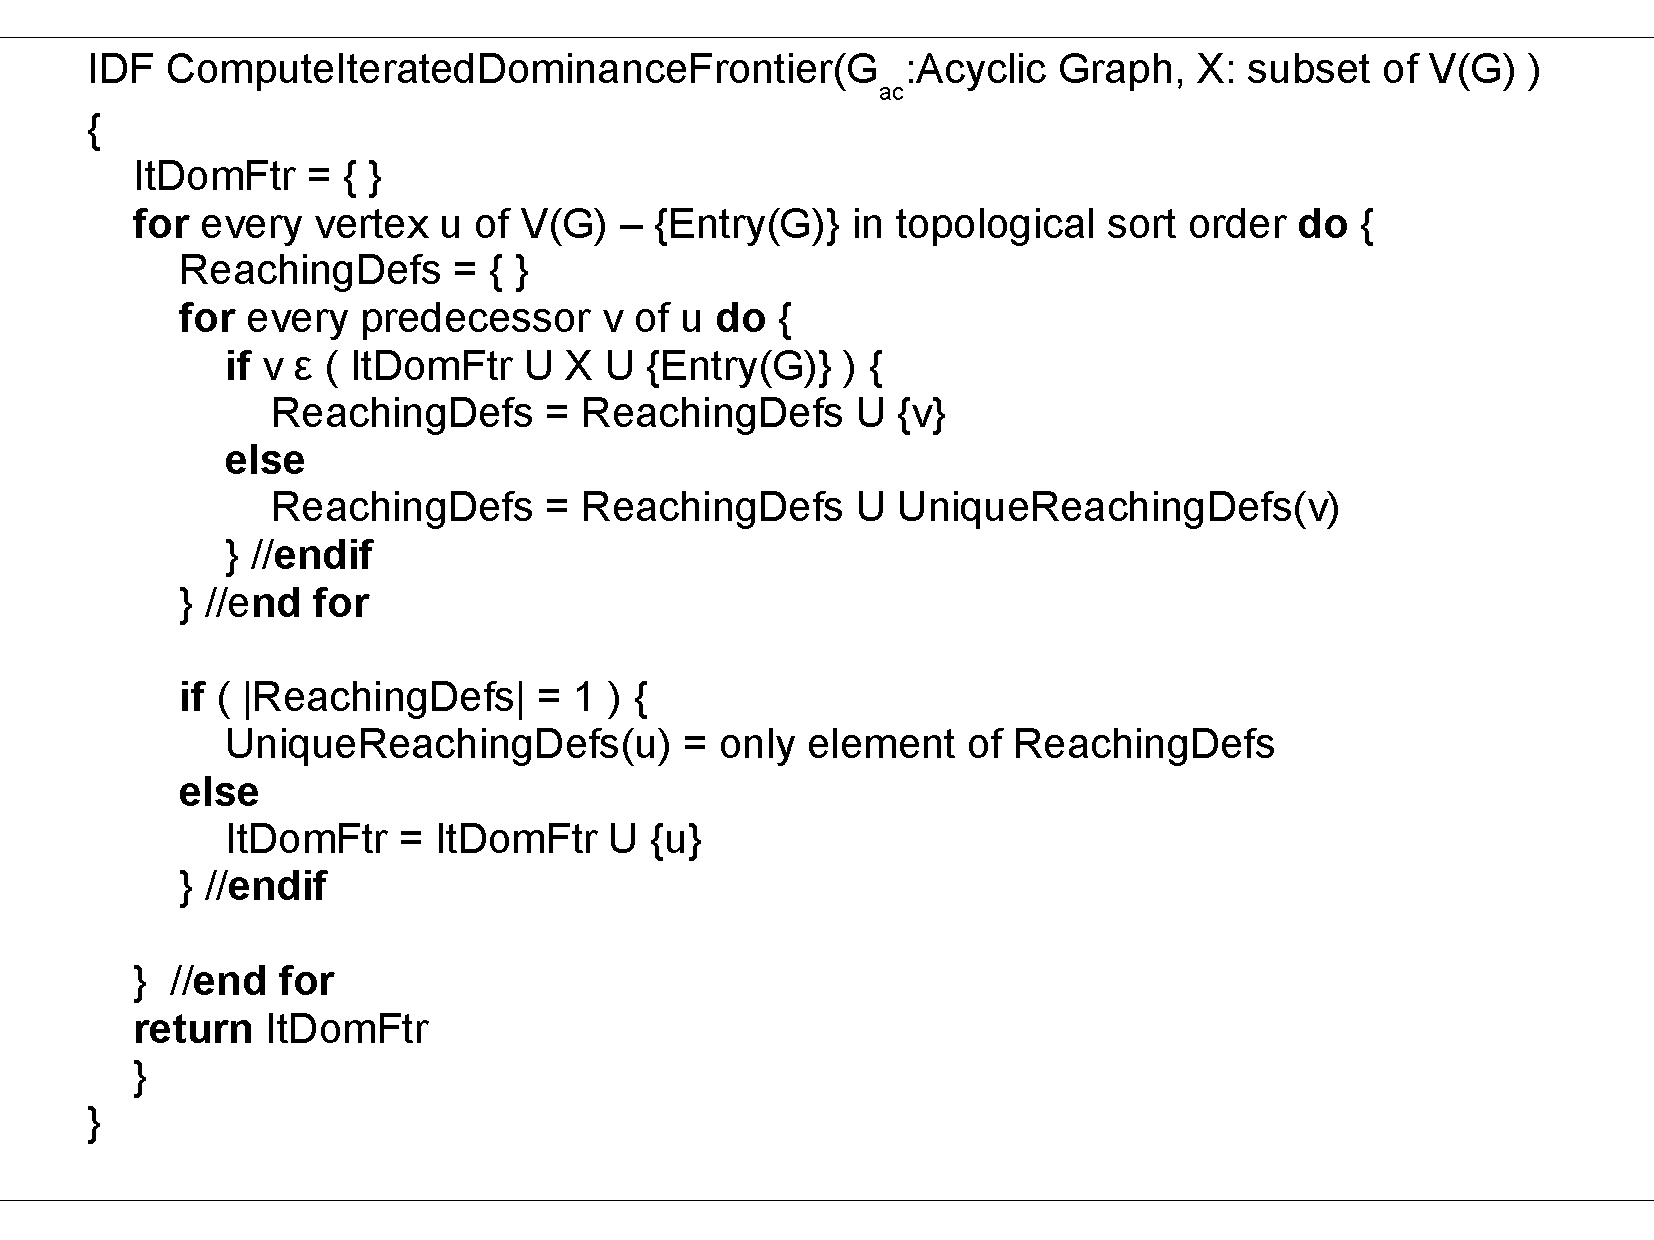
\includegraphics[scale=0.3]{idfcode.pdf}}
    %\caption{Pseudocode for computing IDF of an acyclic graph }
    %\label{fig:idfcode}
    %\end{figure}  
    
   \begin{figure}[!ht]
   \centering
  \begin{minipage}[t]{5in}
  \noindent{\bf Input:} An acyclic CFG $G_{ac}$, $X$: subset of $V(G)$.
  \noindent{\bf Output:} The set $IDF(X)$.
  \setcounter{linectr}{0}

    Procedure ComputeIteratedDominanceFrontier($G_{ac}$:Acyclic graph,$X$: subset of $V(G)$)
    \{
    \begin{code}

    \x1 $IDF = \{ \}$; 
    \x1 $\forall$ $node$ of $V(G)$, $UniqueReachingDefs(node)$ = \{ \};
    \x1 {\bf for} $\forall u$ of $V(G) - entry(G)$ in topological sort order {\bf do} \{ 
    \x2    $ReachingDefs = \{ \}$; 
    \x2    {\bf for} $\forall$ predecessor $v$ of $u$ {\bf do} \{ 
    \x3      {\bf if} $v \in$ ( $IDF \cup X \cup entry(G)$ ) {\bf then} 
    \x4         $ReachingDefs = ReachingDefs \cup \{v\}$; \label{C:rdf}
    \x3      {\bf else} 
    \x4         $ReachingDefs = ReachingDefs \cup UniqueReachingDefs(v)$; \label{C:urdf}
    \x3      {\bf end if} 
    \x2   {\bf end for} 
    \x2   {\bf if} ( $\|ReachingDefs\|$ == 1 ) {\bf then} \label{C:onerd}
    \x3      $UniqueReachingDefs(u) = $ only element of $ReachingDefs$; 
    \x2   {\bf else} 
    \x3       $IDF = IDF \cup \{u\}$; \label{C:ridf}
    \x2   {\bf end if}    
    \x1 {\bf end for} 
    \x1 {\bf return} $IDF$;   
     
    \end{code}
    \}
 
  \end{minipage}
  \caption{Ramalingam's algorithm for computing the IDF of an acyclic graph.}
  \label{F:ramaIDF}
  \end{figure}

    We will walk through some of the steps of this algorithm for $IDF(\{4,5,7,12\})$. We will start at
    vertex 4. For this vertex, ${\it predecessors} = \{3\}$. But as $3 \notin IDF \cup X \cup \{entry\})$, 
    ${\it ReachingDefs} = {\it UniqueReachingDefs}(3)$ according to step ~\ref{C:urdf}. Hence, 
    ${\it ReachingDefs} = \{entry\}$. As $\|{\it ReachingDefs}\|$ equals 1, 
    ${\it UniqueReachingDefs}(4) = \{entry\}$.
    The same logic applies for vertices 5 and 7, and so, 
    ${\it UniqueReachingDefs}(5) = {\it UniqueReachingDefs}(7) = \{entry\}$.
    For vertex 6, ${\it predecessors} = \{4,5\}$.
    Since both vertices 4 and 5 belong to $X$, according to step ~\ref{C:rdf}, 
    ${\it ReachingDefs} = \{4,5\}$.
    As $\|{\it ReachingDefs}\| \neq 1$, according to step ~\ref{C:ridf}, $IDF = \{6\}$.
    Following similar arguments, $IDF = \{6,8\}$, when node 8 is visited. When the rest of the vertices
    are visited, the IDF set remains unchanged. 

    How can the algorithm to find IDF for acyclic graphs be extended to handle reducible graphs? 
    A reducible graph can be
    decomposed into an acyclic graph and a set of backedges. The contribution of backedges to the
    iterated dominance frontier can be identified by using the loop nesting forest. If a vertex $u$
    is contained in a loop then $IDF(u)$ will contain the loop header. For any vertex $u$, let $HLC(u)$
    denote the set of loop headers of the loops containing $u$. Given a set of vertices $X$, it turns
    out that $IDF(X) = HLC(X) \cup IDF_{ac}(X \cup HLC(X))$ where $IDF(X)$ and $IDF_{ac}$
    denote the IDF over the original graph $G$ and the acyclic graph $G_{ac}$ respectively. Reverting
    back to Figure ~\ref{fig:lnf} we see that in order to find the $IDF$ for the nodes where the variable 
    $v$ is defined, we need to evaluate $IDF(\{4,5,7,12\})$. Firstly, we would need to evaluate 
    $IDF_{ac}(\{4,5,7,12\} \cup HLC(\{4,5,7,12\}))$. $HLC(\{4,5,7,12\}) = \{2\}$ as all these nodes are contained 
    in a single loop with header $2$. Hence, we would need to find $IDF_{ac}(\{2,4,5,7,12\})$ which turns
    out to be the set $\{6,8\}$. Finally, $IDF(\{4,5,7,12\}) = HLC(\{4,5,7,12\}) \cup \{6,8\} = \{2,6,8\}$.
 
    %\noindent
    \begin{figure}[htb]
    \centerline{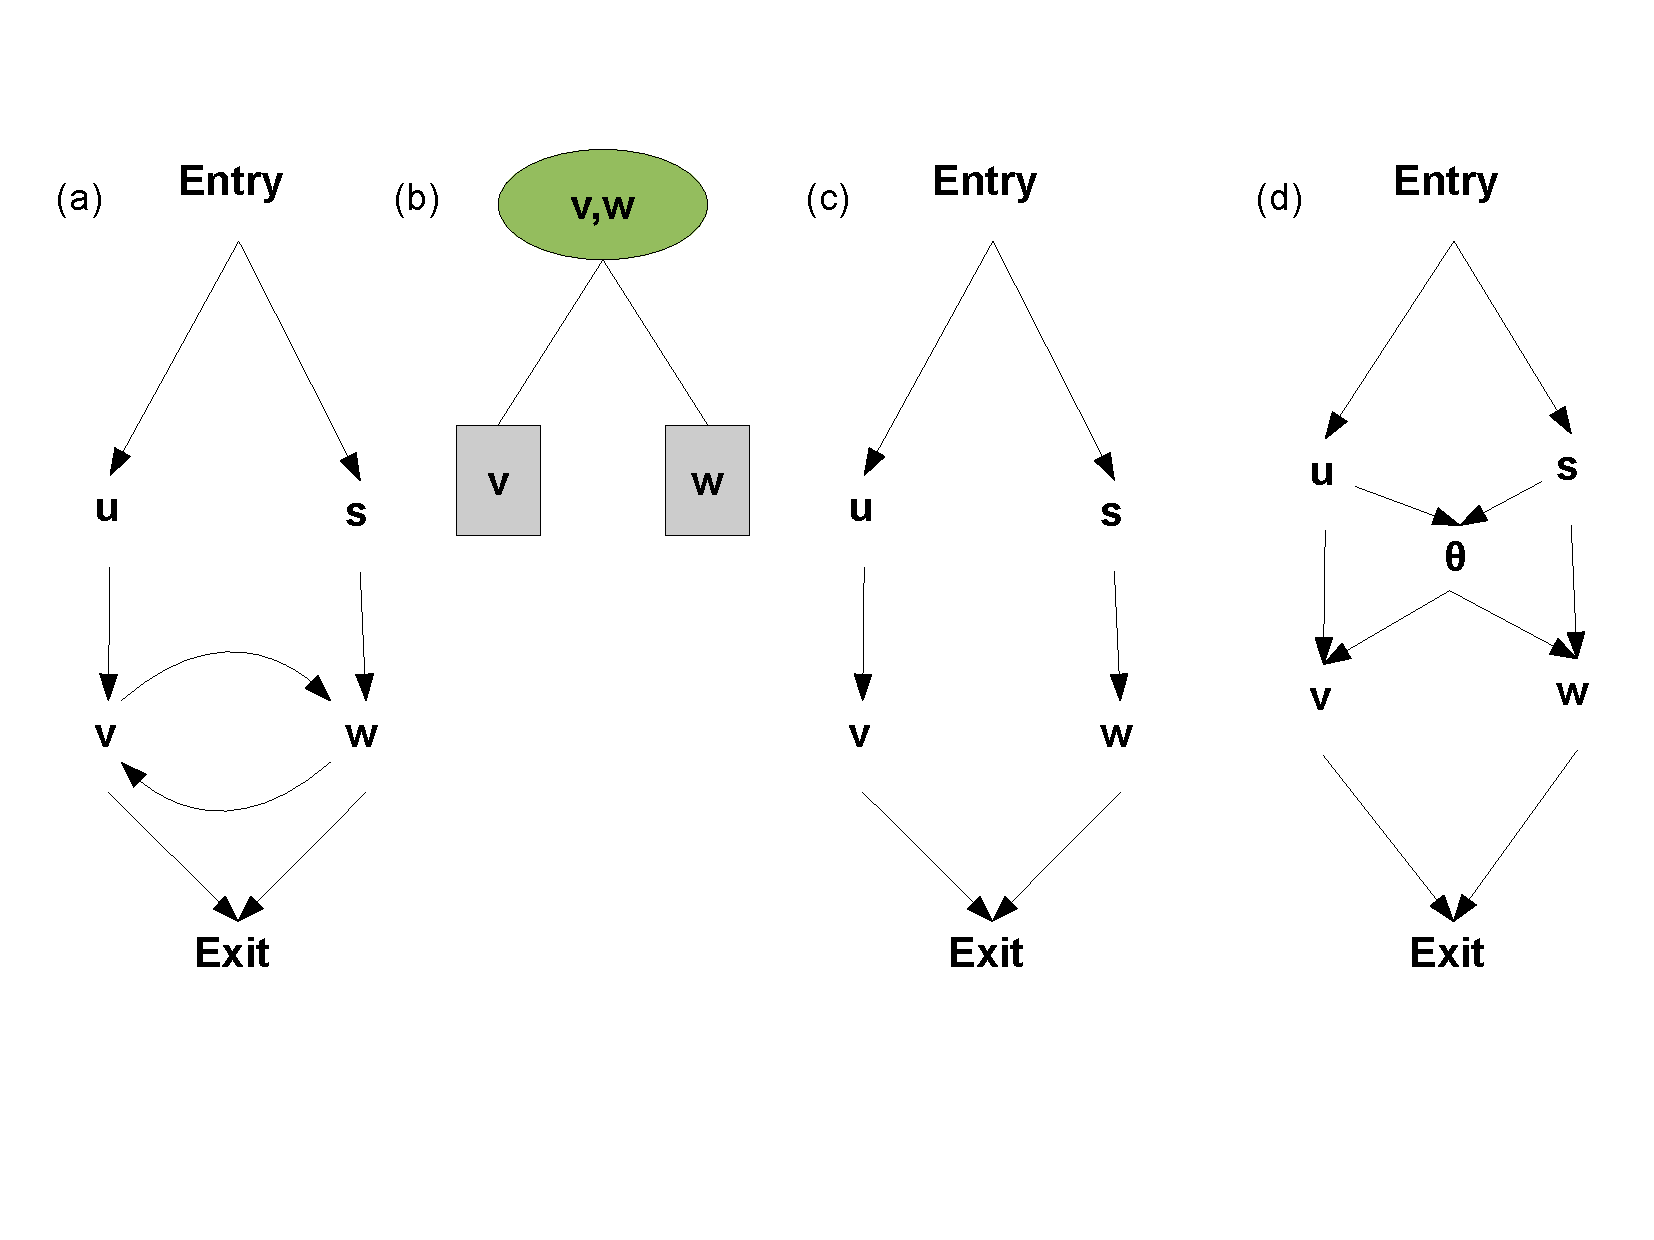
\includegraphics[scale=0.3]{irred.pdf}}
    \caption{(a) An irreducible graph (b) The Loop Nesting Forest (c) The acyclic subgraph (c) Transformed
    graph}
    \label{fig:irred}
    \end{figure} 
 
    Now that we have shown how IDF can be computed for graphs with reducible loops using 
    loop nesting forests, we will briefly touch
    upon how graphs containing irreducible loops can be handled. The trick behind the implementation
    is to transform the irreducible loop in such a way that an acyclic graph is created from the loop
    without changing the dominance properties of the nodes. Referring to Figure ~\ref{fig:irred}, we see 
    that the irreducible loop comprising of nodes $v$ and $w$ in (a) can be transformed to the acyclic
    graph in (c) by removing the edges between nodes $v$ and $w$ that create the irreducible loop. 
    We can now create a new dummy node $\theta$ and add edges from the predecessor of all
    the header nodes of the cycles of the irreducible graph to $\theta$, 
    as well as add edges from $\theta$ to all the 
    header nodes. This results in additional edges from $u$ and $s$ which are the predecessors of the
    header nodes $v$ and $w$ respectively to $\theta$. In addition, extra edges are added from $\theta$
    to the header nodes $v$ and $w$.The transformed graph is shown in (d). Following this transformation, 
    computing IDF for the nodes 
    in the original irreducible graph translates to computing IDF for the transformed graph. Since this
    graph is acyclic, the algorithm depicted in Figure ~\ref{F:ramaIDF} can be applied by noting the
    loop nesting forest structure as shown in (b). The crucial observation that allows this transformation 
    to create an equivalent acyclic
    graph is the fact that the dominator tree of the transformed graph remains identical to the
    original graph containing an irreducible cycle. One of the drawbacks of the transformation is the
    possible explosion in the number of dummy nodes and edges for graphs with many irreducible cycles as
    a unique dummy node needs to be created for each irreducible loop. However, such cases may be rare
    for practical applications.

    \section{Summary}
    This chapter provides an overview of some advanced construction algorithms
    for SSA. These include the first proposed linear-time algorithm by Sreedhar using the concept of
    DJ graphs, the merge relation by Pingali and Bilardi, a DJ graph and merge
    set based algorithm by Das and Ramakrishna and finally an algorithm by Ramalingam based on the concept
    of loop nesting forests. Though all these algorithms claim to be better than the original CFR algorithm, 
    they are difficult to compare due to the unavailability of these algorithms in a common compiler framework.
    However, some of these algorithms are known to perform better than CFR for several well-known benchmarks.


%%%%%%%%%%%%%%%%%%%%%%%%%
%%%%%%%%%%%%%%%%%%%%%%%%%
%%%%%%%%%%%%%%%%%%%%%%%%%


\section{SSA destruction for machine code \Author{F. Rastello}}
\label{sec:advanced_destruction}
\textbf{5 pages}
Describes the context: cannot necessarily split critical edges, some variables have renaming constraints, some instructions have renaming constraints that we want to handle during SSA destruction (some may be handled during register allocation). 

Renaming constraints are handled using copies around constrained instructions. Go to conventional-SSA using Sreedhar's~I technique. Outline the limitation of this technique when dealing with condional jump instruction that define a variable itself; when dealing with renaming constraints for variables that interfere...

Define our ``ultimate'' notion of interference using value. Build the interference graph (provide the simplified pseudo-code). Do coalescing. Refer to CGO'09 paper for issues concerning JIT compilation. Remove $\phi$-functions and perform renaming. Provide a more sophisticated pseudo-code (than for \ref{sec:classical_destruction}) for parallel copies sequentialisation (that can be performed before or after coalescing and $\phi$ removal.

